\documentclass{article}
\usepackage[margin=1in]{geometry}
\usepackage{amsmath,amsthm,amssymb}
\usepackage{bbm,enumerate,mathtools}
\usepackage{tikz,pgfplots}
\usepackage{chessboard}
\usepackage[hidelinks]{hyperref}
\usepackage{multicol} % Problem 35

\newenvironment{question}{\begin{trivlist}\item[\textbf{Question.}]}{\end{trivlist}}
\newenvironment{note}{\begin{trivlist}\item[\textbf{Note.}]}{\end{trivlist}}
\newenvironment{references}{\begin{trivlist}\item[\textbf{References.}]}{\end{trivlist}}
\newenvironment{related}{\begin{trivlist}\item[\textbf{Related.}]\end{trivlist}\begin{enumerate}}{\end{enumerate}}

\usetikzlibrary{decorations.pathreplacing}

\begin{document}

\rating{2}{1}
% Consider Truchet tiles ...
\begin{figure}[ht!]
  \centering
  \noindent
  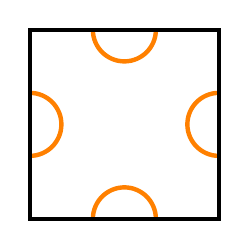
\begin{tikzpicture}[scale=0.8]
    \draw[cyan!0!orange, ultra thick]
      (1,0) arc (180:0:0.5)    % bottom
      (0,1) arc (-90:90:0.5)   % left
      (3,1) arc (270:90:0.5)   % right
      (1,3) arc (180:360:0.5)  % top
    ;
    \draw[ultra thick] (0,0) rectangle (3,3);
  \end{tikzpicture}
  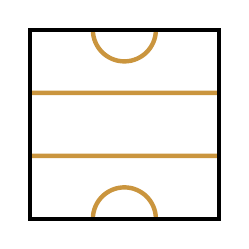
\begin{tikzpicture}[scale=0.8]
    \draw[cyan!20!orange, ultra thick]
      (1,0) arc (180:0:0.5)    % bottom
      (0,1) -- (3,1)
      (0,2) -- (3,2)
      (1,3) arc (180:360:0.5)  % top
    ;
    \draw[ultra thick] (0,0) rectangle (3,3);
  \end{tikzpicture}
  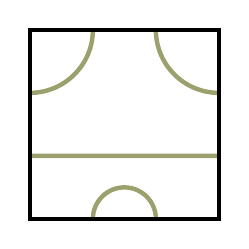
\begin{tikzpicture}[scale=0.8]
    \draw[cyan!40!orange, ultra thick]
      (1,0) arc (180:0:0.5)    % bottom
      (0,1) -- (3,1)
      (0,2) arc (-90:0:1)      % NW
      (3,2) arc (270:180:1)    % NE
    ;
    \draw[ultra thick] (0,0) rectangle (3,3);
  \end{tikzpicture}
  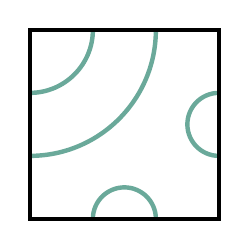
\begin{tikzpicture}[scale=0.8]
    \draw[cyan!60!orange, ultra thick]
      (1,0) arc (180:0:0.5)    % bottom
      (0,2) arc (-90:0:1)      % NW
      (0,1) arc (-90:0:2)      % NW'
      (3,1) arc (270:90:0.5)   % right
    ;
    \draw[ultra thick] (0,0) rectangle (3,3);
  \end{tikzpicture}
  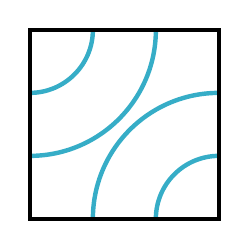
\begin{tikzpicture}[scale=0.8]
    \draw[cyan!80!orange, ultra thick]
      (0,2) arc (-90:0:1)      % NW
      (0,1) arc (-90:0:2)      % NW'
      (2,0) arc (180:90:1)     % SE
      (1,0) arc (180:90:2)     % SE'
    ;
    \draw[ultra thick] (0,0) rectangle (3,3);
  \end{tikzpicture}
  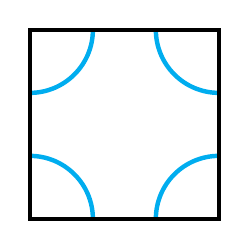
\begin{tikzpicture}[scale=0.8]
    \draw[cyan!100!orange, ultra thick]
      (0,2) arc (-90:0:1)      % NW
      (0,1) arc (90:0:1)       % SW
      (2,0) arc (180:90:1)     % SE
      (2,3) arc (180:270:1)     % NE
    ;
    \draw[ultra thick] (0,0) rectangle (3,3);
  \end{tikzpicture}
  \caption{
    For $(n,k) = (4,2)$, it appears that there are $C(4) = 14$ valid patterns
    in six equivalence classes.
  }
\end{figure}
\begin{figure}[ht!]
  \centering
  \noindent
  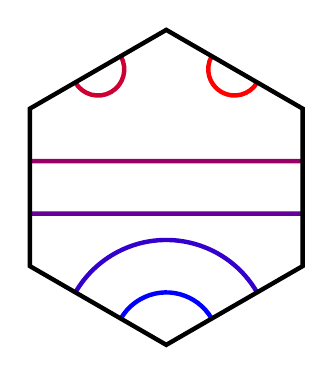
\begin{tikzpicture}[scale=2, rotate=30]
    \draw[red!0!blue, ultra thick] (0.333,0) arc (0:120:0.333);
    \draw[red!20!blue, ultra thick] (0.666,0) arc (0:120:0.666);
    \draw[red!40!blue, ultra thick] (-1/3,{4/3*sqrt(3)/2}) -- (7/6,{sqrt(3)/6});
    \draw[red!60!blue, ultra thick] (-1/6,{5/3*sqrt(3)/2}) -- (4/3,{sqrt(3)/3});
    \draw[red!80!blue, ultra thick] (0.333,{sqrt(3)}) arc (180:360:0.1666);
    \draw[red!100!blue, ultra thick] (4/3,{4/3*sqrt(3)/2}) arc (300:120:0.1666);
    \draw[ultra thick]
      (-0.5, {sqrt(3)/2}) --
      (0,    0          ) --
      (1,    0          ) --
      (1.5,  {sqrt(3)/2}) --
      (1,    {sqrt(3)}  ) --
      (0,    {sqrt(3)}  ) --
      cycle;
  \end{tikzpicture}
  ~
  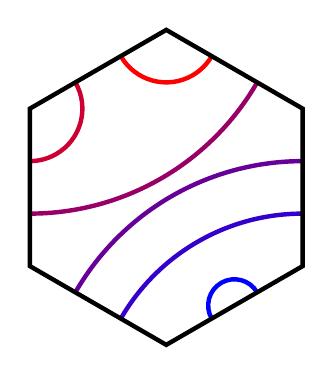
\begin{tikzpicture}[scale=2, rotate=30]
    \draw[red!0!blue, ultra thick] (0.333,0) arc (180:0:0.1666);
    \draw[red!20!blue, ultra thick] (-1/6,{1/3*sqrt(3)/2}) arc (120:60:4/3);
    \draw[red!40!blue, ultra thick] (-1/3,{2/3*sqrt(3)/2}) arc (120:60:5/3);
    \draw[red!60!blue, ultra thick] (-1/3,{4/3*sqrt(3)/2}) arc (240:300:5/3);
    \draw[red!80!blue, ultra thick] (1/3,{sqrt(3)}) arc (0:-120:1/3);
    \draw[red!100!blue, ultra thick] (2/3,{sqrt(3)}) arc (180:300:1/3);
    \draw[ultra thick]
      (-0.5, {sqrt(3)/2}) --
      (0,    0          ) --
      (1,    0          ) --
      (1.5,  {sqrt(3)/2}) --
      (1,    {sqrt(3)}  ) --
      (0,    {sqrt(3)}  ) --
      cycle;
  \end{tikzpicture}
  ~
  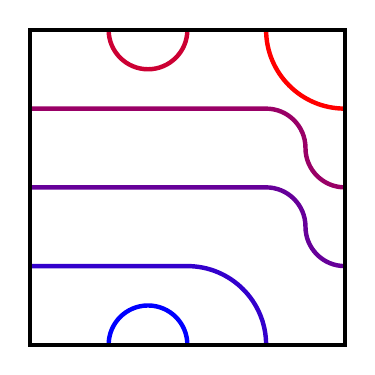
\begin{tikzpicture}[scale=1]
    \draw[red!0!blue, ultra thick]  (1,0) arc (180:0:0.5);
    \draw[red!20!blue, ultra thick]  (3,0) arc (0:90:1) -- (0,1);
    \draw[red!40!blue, ultra thick]   (4,1) arc (270:180:0.5) arc (0:90:0.5) -- (0,2);
    \draw[red!60!blue, ultra thick]   (4,2) arc (270:180:0.5) arc (0:90:0.5) -- (0,3);
    \draw[red!100!blue, ultra thick]   (4,3) arc (270:180:1);
    \draw[red!80!blue, ultra thick]  (1,4) arc (180:360:0.5); % N
    % \draw[red!100!blue, ultra thick] (4,2) arc (270:90:0.5); % E
    \draw[ultra thick] (0,0) rectangle (4,4);
  \end{tikzpicture}
  ~
  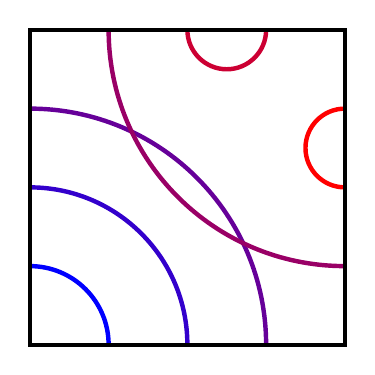
\begin{tikzpicture}[scale=1]
    \draw[red!0!blue, ultra thick]  (1,0) arc (0:90:1);    % SW
    \draw[red!20!blue, ultra thick]  (2,0) arc (0:90:2);    % SW
    \draw[red!40!blue, ultra thick]   (3,0) arc (0:90:3);    % SW
    \draw[red!60!blue, ultra thick]  (1,4) arc (180:270:3); % NE
    \draw[red!80!blue, ultra thick]  (2,4) arc (180:360:0.5); % N
    \draw[red!100!blue, ultra thick] (4,2) arc (270:90:0.5); % E
    \draw[ultra thick] (0,0) rectangle (4,4);
  \end{tikzpicture}
  \caption{
    A valid $(6,2)$-pattern does not always have a corresponding valid
    $(4,3)$-pattern: the first square's pattern has curves that are not line
    segments or circular arcs, and the second square's pattern is self-overlapping.
  }
\end{figure}
\begin{question}
  Given an $n$-gon with $k$ markings on each side, how much such patterns can
  be made using circular arcs and line segments such that each curve meets the
  boundary at a right angle?
\end{question}

\begin{note}
  An $(n,k)$-pattern has or $C(nk/2)$ fewer realizations, where $C(m)$ is the
  $m$-th Catalan number.
\end{note}

\begin{related}
  \item How many $(n,k)$-patterns up to dihedral action of the $n$-gon?
  \item For some fixed $k$, which values of $N$ allow for $C(Nk/2)$ $(N,k)$-patterns?
  If none, what are the obstructions?
  \item How does this generalize to non-regular polygons or to higher dimensional polytopes?
  \item What if curves other than circular arcs and line segments are allowed?
\end{related}

\begin{references}
  \item Problems 28, 31, and 92.
\end{references}
\end{document}
